\documentclass[conference,letterpaper]{IEEEtran}
\IEEEoverridecommandlockouts
\usepackage{cite}
\usepackage{amsmath,amssymb,amsfonts}
\usepackage{graphicx}
\usepackage{textcomp}
\usepackage[OT1]{fontenc}
\usepackage{pifont}
\usepackage{listings}
\lstset{
basicstyle=\small\ttfamily,
columns=flexible,
breaklines=true
}
\usepackage{multirow}
\usepackage{threeparttable}
\usepackage{booktabs}% http://ctan.org/pkg/booktabs
\usepackage{hyperref}
\usepackage{tikz}
\usepackage{geometry}
\usepackage{array}
\usepackage{float}
\geometry{margin=0.6in}
\setlength{\extrarowheight}{5pt}
\columnsep = 0.2in
\usepackage[noend]{algpseudocode}
\definecolor{realBlue}{HTML}{044d97}
\hypersetup{
    colorlinks=false,
    linkcolor=realBlue,
    filecolor=magenta,
    urlcolor=realBlue,
    pdftitle={Domain Name Server Spoofing Using Ettercap And DNSMasq},
    pdfpagemode=FullScreen,
}

\newcommand{\tabitem}{~~\llap{\textbullet}~~}
\newcommand{\etal}{{\em et al.\ }}

\newcommand*{\red}{\textcolor{red}}
\definecolor{LightCyan}{rgb}{0.88,1,1}
\makeatletter
 \newcommand{\linebreakand}{%
 \end{@IEEEauthorhalign}
 \hfill\mbox{}\par
 \mbox{}\hfill\begin{@IEEEauthorhalign}
 }

 \makeatother
\def\BibTeX{{\rm B\kern-.05em{\sc i\kern-.025em b}\kern-.08em
    T\kern-.1667em\lower.7ex\hbox{E}\kern-.125emX}}
\begin{document}
\bibliographystyle{IEEEtran}
\title{Domain Name Server Spoofing Using Ettercap And Dnsmasq}
\author{
\IEEEauthorblockN{Adithya Nair, Avighna Reddy Katipally, P Ananthapadmanabhan Nair}
\textit{Department Of Computer Science And Engineering} \\
\textit{Amrita School Of Computing, Bengaluru} \\
\textit{Amrita Vishwa Vidyapeetham, India} \\
\href{mailto:bl.en.u4aid23002@bl.students.amrita.edu}{bl.en.u4aid23002@bl.students.amrita.edu} \\
\href{mailto:bl.en.u4aid23005@bl.students.amrita.edu}{bl.en.u4aid23005@bl.students.amrita.edu} \\
\href{mailto:bl.en.u4aid23036@bl.students.amrita.edu}{bl.en.u4aid23036@bl.students.amrita.edu} \\
}

\maketitle

\begin{abstract}
The Domain Name System (DNS) represents a foundational yet critically vulnerable component of global internet infrastructure, serving the essential function of translating human-readable domain names into machine-addressable IP addresses. Despite its ubiquity and fundamental role in facilitating internet communication, DNS remains susceptible to sophisticated exploitation techniques that can compromise network security and user safety.
This comprehensive research paper presents an in-depth technical exploration of DNS spoofing, a sophisticated network attack methodology that allows malicious actors to manipulate DNS resolution processes. By establishing a controlled experimental environment using virtualized network resources, we demonstrate the technical intricacies of DNS spoofing attacks, focusing on their implementation, potential impact, and strategic mitigation approaches.
Our experimental methodology leverages virtualization technologies, specifically Oracle VirtualBox\cite{oracleVirtualBoxGeneralpurposeFull}, and employs specialized cybersecurity tools including Kali Linux, Metasploitable, dnsmasq, ettercap, and Wireshark. Through meticulously crafted experiments, we systematically capture, analyze, and deconstruct DNS spoofing attack vectors, providing researchers and cybersecurity professionals with granular insights into these network vulnerabilities.
The research not only illustrates the technical mechanics of DNS spoofing but also critically evaluates multiple mitigation strategies. These include implementing static ARP entries, enforcing trusted DNS server configurations, and exploring encrypted DNS query mechanisms such as DNS-over-HTTPS. By presenting a holistic view of the attack landscape, this study aims to advance understanding of DNS infrastructure vulnerabilities and provide actionable strategies for enhancing network security defenses.
\end{abstract}

\begin{IEEEkeywords}
  DNS Spoofing, Domain Name System, Cybersecurity, Network Exploits, Virtual Machines, Pentesting
\end{IEEEkeywords}

\section{Introduction}

The Domain Name System (DNS) serves as a critical architectural backbone of internet communication, functioning as a distributed, hierarchical naming system that translates human-readable domain names into machine-processable IP addresses. This fundamental protocol enables seamless internet navigation, allowing users to access online resources through intuitive, memorable domain names rather than complex numerical IP addresses.
Implemented through sophisticated software systems like BIND (Berkeley Internet Name Domain)\cite{aliDNSUsingBIND2015}, DNS operates through a complex network of interconnected servers that cache and propagate domain name information. However, this critical infrastructure is inherently vulnerable to various sophisticated exploitation techniques, with DNS spoofing emerging as one of the most prevalent and potentially devastating attack methodologies.
DNS spoofing, alternatively termed DNS cache poisoning, represents a sophisticated network attack where malicious actors manipulate DNS record mappings to redirect network traffic toward unauthorized or malicious IP addresses. The potential consequences of such attacks are profound and multifaceted, including:

\begin{enumerate}
\item Compromising data integrity by intercepting and potentially modifying network communications
\item Facilitating advanced phishing campaigns by redirecting users to fraudulent websites
\item Enabling complex man-in-the-middle attacks that can intercept sensitive information
\item Potentially breaching organizational network security frameworks
\end{enumerate}

This research paper presents a comprehensive, technically rigorous examination of DNS spoofing through a carefully constructed experimental framework. By utilizing virtualization technologies and specialized cybersecurity tools, we aim to provide an empirical demonstration of DNS spoofing mechanics, attack vectors, and potential mitigation strategies.
The experimental setup employs Oracle VirtualBox\cite{oracleVirtualBoxGeneralpurposeFull} to create a controlled network environment, with a Kali Linux virtual machine serving as the attack platform and a Metasploitable virtual machine representing a vulnerable target system. Through the strategic deployment of tools like dnsmasq for rogue DNS server establishment and ettercap for network traffic manipulation, we simulate a realistic DNS spoofing scenario targeting the hypothetical domain grouptwo.com.
By meticulously capturing and analyzing network traffic using Wireshark, our research offers unprecedented insights into the technical execution of DNS spoofing attacks. Moreover, we systematically evaluate and propose multiple mitigation techniques, including static ARP entry configuration, trusted DNS server enforcement, and the implementation of encrypted DNS query protocols like DNS-over-HTTPS\cite{csikorPrivacyDNSoverHTTPSRequiem2021}
The primary objectives of this research are threefold:

\begin{enumerate}
\item\label{item:1}  Demonstrate the technical mechanics of DNS spoofing attacks
  \item Analyze the potential network security implications of such exploits
  \item  Provide actionable strategies for preventing and mitigating DNS infrastructure vulnerabilities
\end{enumerate}

Through this comprehensive exploration, we aspire to contribute to the ongoing dialogue surrounding network security, raise awareness about DNS vulnerabilities, and equip cybersecurity professionals with practical knowledge for defending against these sophisticated attack methodologies.

\section{Implementation}
\subsection{Setup}

We set up \textit{dnsmasq} with the following configuration, where we write a local DNS record stating that grouptwo.com is situated at 10.0.2.15

We do this by updating the \textit{dnsmasq.conf} file.

\begin{lstlisting}
interface=eth0
address=/grouptwo.com/10.0.2.15
\end{lstlisting}

We then update the \textit{etter.dns} file as well. This allows the DNS Spoofing software we are using to log when our DNS server has successfully spoofed a machine.

\begin{lstlisting}
grouptwo.com A 10.0.2.15
\end{lstlisting}

We enable IP forwarding on our VM with the following command. IP Forwarding allows our VM to inspect all packets that come in, tamper with the packets and then send them to their destination address.

\begin{lstlisting}
echo 1 > /proc/sys/net/ipv4/ip_forward
\end{lstlisting}

We update our iptables\cite{purdyLinuxIptablesPocket2004} to route both TCP and UDP traffic directed towards port 53 to be redirected towards our Kali VM. Port 53 is the default used by Domain Name System for communication.

\begin{lstlisting}
sudo iptables -t nat -A PREROUTING -p udp --dport 53 -j DNAT --to-destination 10.0.2.15:53

sudo iptables -t nat -A PREROUTING -p tcp --dport 53 -j DNAT --to-destination 10.0.2.15:53
\end{lstlisting}
The last command is used to rewrite the packet such that the source address seems to come from a legitimate DNS server rather than our malicious local DNS server.
\begin{lstlisting}
sudo iptables -t nat -A POSTROUTING -j MASQUERADE
\end{lstlisting}
\subsection{Execution}
Startup \textit{dnsmasq}, this starts up our small DNS forwarding service at port 53 of the Kali VM's IP.

\begin{lstlisting}
systemctl start dnsmasq.service
\end{lstlisting}

Startup \textit{ettercap}. Ettercap\cite{ornaghiEttercapComprehensiveSuite} is a utility that enables our VM to perform ARP\cite{majidhafathimaSurveyNetworkPacket2021} and DNS Spoofing\cite{babuComprehensiveAnalysisSpoofing2011}. This software scans the network for hosts, and starts monitoring the network for traffic.

\begin{lstlisting}
ettercap -G
\end{lstlisting}



\subsection{Packet Capture}
Packets of the attack, both the DNS request and the response from our malicious Kali VM are captured using Wireshark.

\subsubsection{Request}

\begin{lstlisting}
97	39.532672	10.0.2.4	8.8.8.8	DNS	70	Standard query 0x8dd1 A grouptwo.com
\end{lstlisting}

\subsubsection{Response}

Here's the packet capture summary of

\begin{lstlisting}
99	39.533556	8.8.8.8	10.0.2.4	DNS	86	Standard query response 0x8dd1 A grouptwo.com A 10.0.2.15
\end{lstlisting}

\section{Mitigation Strategies}
We have found four major strategies in helping to mitigate such attacks.

\subsection{Static ARP Entries}

We propose implementing static ARP entries, specifically for the router gateway, like so.

\begin{lstlisting}
arp -s <gateway-ip> <gateway-mac-address>
\end{lstlisting}

Upon doing this, any DNS request that gets redirected will be marked as unexpected. The victim device no longer accepts forged ARP entries. DNS requests are sent only to the MAC address of the legitimate DNS server. Any mismatch between the attacker’s spoofed IP and MAC causes DNS queries to fail, effectively blocking the attack.\cite{dataDefenseARPSpoofing2018}

\begin{figure}[ht]
  \centering
  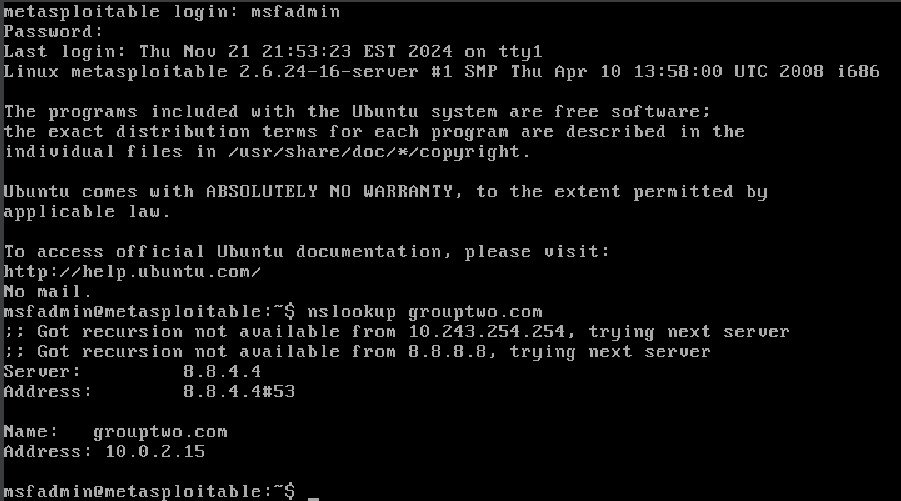
\includegraphics[width=0.5\textwidth]{figures/output.jpeg}
  \caption{Output given by Metasploitable}
\end{figure}


This technique is effective because ARP spoofing operates at the local network level, and static ARP enforces strict control over IP-MAC mappings.\cite{trabelsiARPSpoofingComparative2009}
\subsection{Arp Detection Tooling}

Tools such as \textit{arpwatch} \cite{sudhakarSurveyComparativeAnalysis2017} can be used to monitor traffic and IP-MAC mappings, such tools can generate a log of any changes in IP-MAC addresses and send these logs via email to the administrator

\subsection{Enforce Trusted DNS Servers}

Using DHCP, we can ensure that all devices are configured to a trusted DNS server, such as 1.1.1.1, 8.8.8.8 or an organizational DNS server.

\subsection{DNS Over HTTPS}
Encrypts DNS queries by using HTTPS (Hyper Text Transfer Protocol Secure)\cite{maksutovDetectionPreventionDNS2017}\cite{csikorPrivacyDNSoverHTTPSRequiem2021} to prevent attackers from intercepting or tampering with them, which can be done like so:

\begin{lstlisting}
curl -H 'accept: application/dns-json' 'https://1.1.1.1/dns-query?name=grouptwo.com&type=A'
\end{lstlisting}

Although this isn't perfect, as argued by \cite{csikorPrivacyDNSoverHTTPSRequiem2021}. It's a better solution than current methods of DNS Resolution.

\section{Conclusion}
DNS Poisoning is a serious attack that can be performed on local networks which can lead to large amounts of personal data theft or compromise entire organizations. It is paramount to understand strategies for mitigation as well as understanding the attack vectors through which this takes place. Our work has shed light on the attack and the methodology for implementing it.

\section{Future Work}
This study focused on implementing and mitigating DNS spoofing within a controlled virtual network. While the experiment successfully demonstrated the attack and evaluated mitigation strategies, several avenues for future research and exploration remain:

\begin{enumerate}
  \item Future work can expand the attack methodology to include advanced techniques, such as DNS cache poisoning\cite{trostleProtectingDNSCache2010} at a higher network level (e.g., ISP-level attacks) or combining DNS spoofing with other exploits like phishing or malware delivery to study their compounded effects.\cite{alharbiDNSPoisoningOperating2022}
  \item The experiment was conducted in a simple NAT-based virtual network. Future studies could examine DNS spoofing in more complex setups, involving more end devices, including corporate networks, cloud-based environments, or networks with active intrusion detection systems (IDS) and intrusion prevention systems (IPS).
  \item Developing and testing automated systems that detect DNS spoofing attempts in real-time, using tools like machine learning models trained on data logs and labelled verified logs of attacks to identify anomalies in DNS traffic, could significantly enhance defensive capabilities.
\end{enumerate}

\section{Acknowledgments}
We would like to take this opportunity to thank our professor and mentor, Mr. Vishwas H.N. His guidance provided for the project allowed us to achieve and implement this attack. The insights that he provided through the lectures allowed us to have a solid foundation to explore and understand this avenue of cybersecurity and network vulnerabilities.

\bibliography{networks}

\end{document}
